\chapter[The Higgs boson]{The Standard Model of particle physics and the Higgs boson}

In the current understanding of particle physics, elementary particles are described as excitations of their peculiar fields, a description derived from quantum mechanics, and their interaction are governed by a Lagrangian. In this scheme each fundamental force is associated to a field and its particle(s), which have integer spin value (gauge bosons). 
Conserved physical observables (particle's quantum numbers) are preserved by dedicated gauge symmetries introduced in the Lagrangian. Back in the 1960's, the behavior of the weak force, responsible for the $\beta$ decays and, more generally, for all the decays with long lifetime observed in nature (e.g. the decay of the muon), could not fit in this description. Due to its long lifetime and short interaction distance, the weak force mediator had to be massive, but the direct introduction of a mass term for a bosonic field would have lead to a disruption of the Lagrangian gauge symmetry. 

In this period the work of several physicists, including Peter Higgs and Francois Englert, led to a different formulation of the origin of gauge boson masses, compliant with the requirements of a gauge-invariant Lagrangian. This breakthrough consolidated the model by predicting a new elementary particle: the Higgs boson.

In the first part of this chapter the mathematical formulation of the elementary particles and interactions, the so-called \emph{Standard Model} (SM) of particle physics, is reviewed. In the second part a detailed review of the status of experimental Higgs boson studies is presented.

\section{The Standard Model}
\subsection{Elementary particles}

Elementary particles composing matter are \emph{fermions}, i.e. particles with spin 1/2 which obey the Fermi-Dirac statistics. These particles can be divided into two categories according to their interaction with the strong force (described later): leptons and quarks. The former are neutral with respect to the strong force, while the latter carry a strong charge, the so-called "color". Quarks and leptons are divided into three families (or generations). Each family contains a doublet of either quarks or leptons which carry the same quantum numbers as their homologous in the other families. The only distinctive characteristic between families is the mass of their components.

In addition, for each particle there is a corresponding antiparticle. Each anti-matter particle carries the same mass, spin and lifetime as its counter-parts, but has opposite quantum charges.

\paragraph{Leptons} 

Leptons comprise three charged particles, the electron ($e\-$), the muon ($\mu\-$), and the tau ($\tau\-$), all carrying the same electric charge as the electron: $Q = -e = -1.602 \times 10^{-19}$ C. Each of the charged leptons is associated to a \emph{neutrino}, a particle with neutral charge assumed to be massless in the SM. The recent evidence of neutrino oscillations~\cite{Agafonova:2010dc} proved that neutrinos do have a mass, albeit extremely small ($< 2$~eV~\cite{pdg}). The precise values of the neutrino masses are not yet measured. The existence of a fourth lepton family with neutrinos below 45~GeV has been excluded by the fit of the $\Z$ to invisible production at LEP~\cite{ALEPH:2005ab}. 

\paragraph{Quarks}

Quarks carry fractional electric charge with respect to the charge of the electron. They also carry a quantum number, called \emph{color}, which allows them to interact with the strong force. The peculiar behavior of the strong force \emph{confines} the quarks within aggregates of multiple constituents called \emph{hadrons}, making impossible the observation of ``independent'' (or ``naked'') quarks. Quarks and anti-quarks cluster in groups of two or three particles, forming \emph{mesons} and \emph{baryons}, respectively. The existence of aggregates of four and five (anti-)quarks, called \emph{tetraquarks} and \emph{pentaquarks}, has been long postulated and only recently confirmed by the BELLE \cite{Choi:2007wga} and LHCb collaborations \cite{Aaij:2014jqa}.

Each quark family is composed by a quark with charge +2/3 and one of charge -1/3 also named ``up-type'' and ``down-type'' respectively from the name of the constituents of the first family (which form protons and neutrons). The presence of a fourth generation of leptons and quarks has not been completely excluded and is object of dedicated searches that are beyond the scope of this work.

Table \ref{tab:quark_leptons} summarizes the properties of the quarks and the leptons currently known.

\begin{table}
\caption{Fundamental particles of the SM, listed with their main properties and classification. For each particle a corresponding anti-particle exists, with same mass and opposite electric charge.}
\label{tab:quark_leptons}
\resizebox{0.9\textwidth}{!}{\begin{minipage}{\textwidth}
\begin{center}
\begin{tabular}{ c|c|c c c c}
\hline
 & Generation & Name & Symbol & Charge [$e$] & Mass [MeV] \\
\hline
\multirow{6}{*}{leptons} & \multirow{2}{*}{1} &  electron & $e$ & -1 & 0.511 \\
  &  &  electronic neutrino & $\nu_e$ & 0 & $< 2 \times 10^{-6}$ \\
\cline{2-6}
  & \multirow{2}{*}{2} &  muon & $\mu$ & -1 & 105.7 \\
  &  &  muonic neutrino & $\nu_\mu$ & 0 & $< 0.19$ \\
\cline{2-6}
  & \multirow{2}{*}{3} &  tau & $\tau$ & -1 & $1.78 \times 10^3$ \\
  &  &  tauonic neutrino & $\nu_\tau$ & 0 & $< 18.2$ \\
\hline
\multirow{6}{*}{quarks} & \multirow{2}{*}{1} &  up & $u$ & $+2/3$ & $2.3^{+0.7}_{-0.5}$ \\
  &  &  down & $\nu_e$ & $-1/3$ & $4.8^{+0.5}_{-0.3}$ \\
\cline{2-6}
  & \multirow{2}{*}{2} &  charm & $c$ & $+2/3$ & $(1.275\pm0.025) \times 10^3$ \\
  &  &  strange & $s$ & $-1/3$ & $95\pm5$ \\
\cline{2-6}
  & \multirow{2}{*}{3} &  top & $t$ & $+2/3$ & $(173.07 \pm0.52 \pm0.72) \times 10^3$ \\
  &  &  bottom/beauty & $b$ & $-1/3$ & $(4.18 \pm0.03) \times 10^3$ \\
\hline
\end{tabular}
\end{center}
\end{minipage}
}
\end{table}


\subsection{Elementary forces}

Elementary forces are mediated by bosons, particles with integer spin. The forces considered fundamental in the SM are:

\paragraph{The \emph{strong} interaction}It is responsible for confining the quarks within the hadrons. It also binds protons and neutrons inside the atomic nuclei. The color charge, linked to the strong interaction, can be defined in a three dimensional group. Unitary charges for the strong interaction are therefore named according to the three primary colors: red, green, and blue. Anti-colors can be defined as negative values of the fundamental color charges. The strong interaction is mediated by eight electrically neutral and massless bosons called \emph{gluons}, each carrying a pair of color and anti-color charges. The peculiar characteristic of the strong interaction, which differentiates it from the other fundamental forces, is that its strength grows as  the distance between the interacting particles increases, leading to the confinement of the quarks. A hadron, globally neutral with respect to strong interaction, it is often referred as ``white'' due to optical color analogy.

\paragraph{The \emph{electromagnetic} (EM) interaction}It is responsible for the reactions between electrically charged particles, and is empirically known to have an infinite range. The part of the SM that describes this interaction is called \emph{Quantum Electrodynamics} (QED) and considers the interaction to be mediated by massless neutral particles called \emph{photons}, which are the EM wave quanta.

\paragraph{The \emph{weak} interaction}It is responsible for most of the nuclear decays that can be observed in nature (except the $\alpha$ and $\gamma$ nuclear decays). Its short interaction range and relative long lifetime of particles decaying weakly, such as the muon, imply the mediators to be massive. The weak interaction allows for decays that are forbidden by the strong and EM interactions, such as flavor-changing decays (i.e. between different generations) and parity-violating decays. The weak interaction is mediated by two charged bosons, the $\W^\pm$, of mass $m_\W = 80.4$ GeV and a neutral boson, the $\Z\0$, of mass $m_\Z = 91.2$ GeV.

\paragraph{The \emph{gravitational} interaction}It is responsible of the attraction between bodies. It is expected to be mediated by a spin 2 boson called the \emph{graviton}. No experimental evidence has been found for the existence of such particle, however. The gravitational force is not included in the SM as its strength is so faint its effect on fundamental particles is not measurable with present-day experiments. % and no clear theory has yet managed to couple the quantum field theory framework with the general relativity one.
A summary of the interactions is given in Table \ref{tab:bosons}.

%\begin{savenotes}
\begin{table}
\caption{Fundamental interactions and their main properties.}
\label{tab:bosons}
%\resizebox{0.9\textwidth}{!}{\begin{minipage}{\textwidth}
\begin{center}
\begin{tabular}{ c c c c c c}
\hline
Interaction & Effective coupling & Mediator & Mass [GeV] & Range [fm]\\
\hline
Gravitation & $10^{-39}$ & graviton & 0 & $\inf$ \\
Electromagnetism & $1/137$ & photon & 0 & $\inf$ \\
Weak force & $10^{-5}$ & $\W^\pm,\Z$ & $80.4,\,91.2$ & $10^{-3}$ \\
Strong force & $1$ & gluon & 0 & $<1$\tablefootnote{The range of the nuclear force, not that of the quark-quark force} \\
\hline
\end{tabular}
\end{center}
\end{table}
%\end{savenotes}

\subsection{A gauge theory of particle interactions}

As briefly outlined in the introduction, the interaction between fundamental particles is described by the Lagrangian formalism. The sum of the charges under a specific interaction is seen as a conserved quantity. In order to protect this quantity a dedicated symmetry is introduced in the form of a local \emph{gauge symmetry}. 

In analogy with the Lagrangian formalism in classical mechanics, the conserved quantity is the generator of the system symmetry. A Noether current is also associated to each charge and symmetry of the Lagrangian. The quantization of this symmetry leads to the presence of a vectorial field. 

For each gauge symmetry exists an associated Lie group. Each of the fundamental particles and force mediators correspond to one of the fundamental representations of the Lie group, fully determining the behavior of the final theory.

The behavior of a free fundamental particle of spin $^1/_2$ is described by the Dirac Lagrangian:

\begin{equation}
\l=\bar{\psi}(i\slash{\d}-m)\psi,
\label{eq:dirac_lag}
\end{equation}

where $\slash{\d} = \gamma^\mu \d_\mu$ and $\psi$ is the particle spinor. % and the slash symbol represent the contraction with a $\gamma$ matrix. 

From the Dirac Lagrangian it is possible to derive the Dirac equation:

\begin{equation}
i \d_t\psi = H \psi,
\label{eq:dirac_lag}
\end{equation}

where $H$ is the free Hamiltonian associated to the Lagrangian.
In this framework the electromagnetic interaction can be described by the U(1) Lie group, whose associated symmetry is a phase change of the spinorial field: % associated to the fundamental particles:

\begin{equation}
\psi'(x) = e^{iq\theta}\psi(x),
\end{equation}

where $q$ denotes the electric charge.
A charged particle is represented by a complex field and the spin behavior is handled by the $\psi$ spinor.

The behavior of a free photon, the gauge boson associated to the electromagnetic force, is described by the Lagrangian:

\begin{equation}
\l = -\frac{1}{4}F_{\mu\nu}F^{\mu\nu},
\end{equation}

where

\begin{equation}
 F_{\mu\nu} =\partial_{\mu}A_{\nu}-\partial_{\nu}A_{\mu}
\end{equation}

and $A_{\mu}$ is the field associated to the photon.
The minimal coupling between a spinor and a photon field is described by the interaction Lagrangian:

\begin{equation}
\l = iq \bar{\psi} \slash{A} \psi.
\end{equation}

The full electromagnetic Lagrangian can therefore be written as:

\begin{equation}
\l_{QED} = \bar{\psi}(i\slash{\calD} - m)\psi - \dfrac{1}{4} F_{\mu\nu} F^{\mu\nu},
\end{equation}

where $\slash{\mathcal{D}} = \d_\mu + i q A_\mu$ is the extension of the four-dimensional derivative $\d$ to ensure the covariance of the Lagrangian. This covariant derivative also embeds the interaction term between the fermions and the photon.

The strong interaction is described by the SU(3) group and its associated gauge symmetry, which is generated by the Gell-Mann matrices, $\tau_a$. A fundamental property of such group is that it is not \emph{abelian}, i.e. the generator matrices do not commute. The commutation rules of the SU(3) group, as any other Lie group, are determined by its \emph{structure constants} $[\tau_a, \tau_b] = i C_{abc} \tau^c$. This property leads to small modification of gauge bosons Lagrangian (Eq. \ref{eq:qcd_free}) and of the coupling with the quarks (Eq. \ref{eq:qcd_int}).

\begin{equation}
\l_{gluons} = - \dfrac{1}{4} G^{a}_{\mu\nu}  G_{a}^{\mu\nu}, \, \rm{with} \, G^{a}_{\mu\nu} = \d_\mu G^a_\nu - \d_\nu G^a_\mu + g_s C_{abc} A^b_\mu A^c_\nu
\label{eq:qcd_free}
\end{equation}

where $A^c_\nu$ is the field associated to the gluon.

\begin{equation}
\l_{quarks} = \bar{\psi} \big( i (\slash{\d} + i g_s \slash{G}^a \tau_a) - m \big) \psi = \bar{\psi} ( i \slash{\calD} - m ) \psi.
\label{eq:qcd_int}
\end{equation}

The presence of trilinear and quartic terms in Eq. \ref{eq:qcd_free} describe the self-interaction between gluons, which is allowed already at the first order of perturbative expansion (also referred as \emph{tree level} or \emph{Born approximation}). The field theory describing strong interactions is called \emph{quantum chromodynamics} (QCD).

\subsection{Discrete and continuous symmetries}

In addition to the gauge symmetries described in the previous section, three discrete symmetries are of particular interest in quantum field theory: charge conjugation (C), parity (P), and time reversal (T). The properties of these symmetries are more easily described by their effect on a quantum state $\ket{f(\vec{p}, h)}$ containing a single particle $f$ of momentum $\vec{p}$ and helicity $h = \vec{s} \cdot \vec{p} / p$, i.e. the projection of the spin along the direction of motion.

The charge conjugation operator C inverts the charge of such state transforming it in its anti-particle: $C\ket{f(\vec{p}, h)} = \eta_C\ket{\anti{f}(\vec{p}, h)}$, where $\eta_C$ is a phase factor. The parity operator P inverts the spatial coordinates, it is often referred as the left-right symmetry: $P\ket{f(\vec{p}, h)} = \eta_P\ket{f(-\vec{p}, -h)}$, where $\eta_P$ denotes the parity of the particle. The time inversion operator T inverts time leading to: $T\ket{f(\vec{p}, h)} = \eta_T\ket{f(-\vec{p}, h)}^*$, where $\eta_T$ is a phase factor depending on the spin of the particle.

Both electromagnetic and strong interaction preserve these three symmetries, while the weak force was experimentally found to violate the charge and parity conjugations. Moreover in 1964 the first experimental evidence of CP (charge and parity combined) violation in K meson decays \cite{PhysRevLett.13.138} was reported. The weak force was found to couple only to ``left-handed'' particles, i.e. particles with negative helicity. More recently the same effect has been found in B mesons decays and is still currently a lively field of study. 

Up to now no evidence of CPT violation has been experimentally observed. An hypothetical observation of CPT violation would have very strong consequences in our understanding of the underlying structure of the fundamental interaction, as this symmetry forbids particles and anti-particles to have different mass or lifetime. The CPT conservation is linked to the statistics to which fermions and bosons obey.

\section{The electroweak force}

In the Standard Model Lagrangian presented so far, the weak force has not been discussed yet. The nature of this interaction has been in fact extremely difficult to model in a quantum field theory framework.

The first attempt to describe the weak interaction dates back to 1933 by Fermi, who suggested for the muon decay the following interaction Lagrangian:

\begin{equation}
\l_{Fermi} = \sqhalf G_F \bar{\nu}_\mu \gamma_\alpha (1-\gamma^5) \mu \bar{e} \gamma^\alpha (1-\gamma^5) \nu_e,
\label{eq:l_fermi}
\end{equation}

where $G_F = 1.166 \cdot 10^{-5}$ GeV$^{-2}$. This Lagrangian consists of a single point-like interaction among four fermions and correctly reproduces the muon decay at tree level. Increasing the degree of the perturbative expansion, though, several divergencies arise that cannot be cancelled or renormalized, leading to a violation of unitarity and a breakdown of the theory. It has also been demonstrated that this behavior can be immediately recognized by the dimensionality of the coupling constant.

It was later shown by Glashow in 1961 \cite{Glashow:1961tr}, and Salam and Ward \cite{Salam:1961en} in the same year, that the weak interaction could be described in a quantum field theory with the SU(2) group and its related gauge bosons. 
The four-fermion interaction in Eq. \ref{eq:l_fermi} is divided into two interaction vertices connected by gauge vector bosons, the W$^\pm$ and the $\Z^0$. In order to obtain the same parity violating properties as observed in the experiments, the gauge group had to be extended to SU(2)$\times$U(1), introducing a mixing between the gauge bosons. This theory showed to represent not only the weak interaction, but also the electromagnetic one. 
The new modeling of these fundamental interactions was finally completed by Weinberg in 1967 \cite{Weinberg:1967tq}, who named it \emph{electroweak theory}. 
As the weak interaction couples only to left-handed particles, the gauge group is sometimes noted as SU(2)$_L$, to remind this feature.

Since the generator of the fundamental representation of SU(2) are the Pauli matrices (noted as $\sigma_i$, $i \, \epsilon \, [1,3]$) it is possible to extend the spin formalism to the weak interaction. In this case the quantum number (or charge) carried by the fundamental particles is called \emph{weak isospin}, noted with I. The gauge bosons linked to the generators of the symmetry will be represented as $W^i$. Left-handed fermions are considered to carry total isospin 1/2 and are grouped in doublets of the form:

\begin{equation}
L_f = \left(\begin{array}{c}f_{up} \\f_{down}\end{array}\right).
\end{equation}

Doublets can be divided in ``up-type'' and ``down-type'' fermions, where the former are considered to have the third component of the isospin I$_3 = +1/2$, while the latter have I$_3 = -1/2$. Up-type fermions are the neutrinos and the up, charm and top quarks, while down-type fermions are the charged leptons and the down, strange, and bottom quarks.

The right-handed fermions were experimentally found not to interact weakly and therefore carry no charge. They are represented as singlets under the SU(2) group.

Left- and right-handed components of the fermions can be obtained by using the appropriate projector on the fermionic spinor: $\dfrac{1}{2}(1-\gamma^5)$ and $\dfrac{1}{2}(1+\gamma^5)$, respectively.

It is worth noting that quark flavor eigenstates under the weak interaction are not necessary also mass eigenstates, but rather a superimposition of them, giving raise to a mixing matrix. The mixing matrix has first been suggested by Cabibbo in 1963 \cite{Cabibbo:1963yz} and by Kobayashi and Maskawa in 1973 \cite{Kobayashi:1973fv}.

The additional U(1) symmetry preserves a quantum number called \emph{hypercharge}, Y, and is connected to a gauge boson, noted with $B$. 

In this framework the derivative present in the Dirac Lagrangian, Eq. \ref{eq:dirac_lag}, is replaced by its covariant form:

\begin{equation}
\calD^L_\mu = \d_\mu - ig\dfrac{\sigma_i}{2}W^i_\mu - ig'\dfrac{Y}{2}B_\mu.
\end{equation}

Since the transformations under SU(2) and U(1) are independent, two coupling constants, $g$ and $g'$, are assigned. The Lagrangian therefore becomes:

\begin{equation}
\l = \sum^f i \bar{L_f}\slash{\calD}^LL_f + \bar{f^{up}_R}\slash{\calD}^Rf^{up}_R  + \bar{f^{down}_R}\slash{\calD}^Rf^{down}_R,
\end{equation}

where $f^{up}_R$ and $f^{down}_R$ are the right-handed up and down fermion field spinors, respectively. Since $f^{up}_R$ and $f^{down}_R$ are singlets under SU(2) they are presented separately, but they still transform under U(1). To account for this effect we have defined $\calD^R = \d_\mu - ig'YB_\mu/2$, which is the same as $\calD^L$, but lacks the couplings with the $W$ fields. 

We can now restrict ourselves to the electron family, without losing any generality, and identify in the Lagrangian a charged and a neutral current:

\begin{eqnarray}
\l_{charged} &=& g \bar{L} \slash{W}_1 \dfrac{\sigma_1}{2}L + g \bar{L} \slash{W}_2 \dfrac{\sigma_2}{2}L, \\ 
\l_{neutral} &=& \dfrac{g}{2} W_3^\mu (\bar{\nu}_{e,L}\gamma_\mu\nu_{e,L} - \bar{e}_L\gamma_\mu e_L) +  \nonumber \\
& & + \dfrac{g'}{2} B^\mu \mathbf{\big(} Y(L) ( \bar{\nu}_{e,L}\gamma_\mu\nu_{e,L} + \bar{e}_L\gamma_\mu e_L ) + \nonumber \\
& & + Y(\nu_R) \bar{\nu}_{e,R}\gamma_\mu\nu_{e,R} + Y(\nu_R)  \bar{e}_R\gamma_\mu e_R \mathbf{\big)}
\end{eqnarray}

The charged part of the Lagrangian contains off-diagonal Pauli matrices that mix the neutrino and electron fields. By means of the substitution:

\begin{equation}
W^\pm_\mu = \frac{1}{\sqrt{2}}(W^{1}_{\mu} \mp i W^{2}_{\mu}),
\label{eq:wpm_def}
\end{equation}

it is possible to rewrite the charged part of the Lagrangian as:

\begin{equation}
\l_c = \frac{g}{\sqrt{2}}(\bar{L}\slash{W}^{+} \sigma^{+} L +\bar{L}\slash{W}^{-}\sigma^{-} L),
\end{equation}

where:

\begin{equation}
\sigma^+ = \spinmatrix{0}{1}{0}{0},\,\, \sigma^- = \spinmatrix{0}{0}{1}{0}.
\end{equation}

In the neutral part of the Lagrangian, neither $W^3$ nor $B$ can be directly identified with the photon, since they both interact with the neutrino which has no electric charge. As the two gauge bosons have the same quantum numbers ($Q = 0$ and $J^P = 1^-$), it is possible to create a linear combination of the two fields which represent the electromagnetic photon.

\begin{equation}
\left\{\begin{matrix}
B^{\mu}=A^{\mu}\operatorname{cos}\theta_{W}-Z^{\mu}\operatorname{sin}\theta_{W}\\ 

W^{\mu}_3=A^{\mu}\operatorname{sin}\theta_{W}+Z^{\mu}\cos\theta_{W}\\ 
\end{matrix}\right.
\label{eq:su2_rotation}
\end{equation}

This linear combination can be seen as a rotation of the fields by an angle $\theta_W$, which is referred to as \emph{Weinberg angle} in the literature. 
The neutral part of the Lagrangian therefore becomes:
 
\begin{equation}
\l_{N}=\bar{\Psi}\gamma_{\mu}(g\operatorname{sin}\theta_{W}T_3+ \frac{Y}{2}g'\operatorname{cos}\theta_{W})\Psi A^{\mu}+\bar{\Psi}\gamma_{\mu}(g\operatorname{cos}\theta_{W}T_3- \frac{Y}{2}g'\operatorname{sin}\theta_{W})\Psi Z^{\mu},
\end{equation}

where:

\begin{equation}
\Psi = \begin{pmatrix}
\nu_L\\ 
e_L\\ 
\nu_R\\ 
e_R
\end{pmatrix}, \, \, \, T_3 = \rm{diag}\left(\frac{1}{2},-\frac{1}{2},0,0\right).
\end{equation}

In this Lagrangian the boson $A$ can be identified with the QED photon. Similarly to what happens to the fields, the electric charge can be written as a linear combination of the third component of the weak isospin and the hypercharge. The charge operator can be derived from the coupling of the photon field to the fermions: 

\begin{equation}
Q = T_3 + \dfrac{Y}{2}.
\end{equation}

In the case of the electron family this leads to the relation:

\begin{equation}
g \opname{sin}\theta_W = g' \opname{cos}\theta_W = e,
\end{equation}

which links the coupling constants and the electron charge to the value of $\theta_W$. The sine and cosine of the Weinberg angle can therefore be defined as:

\begin{equation}
\begin{matrix}
\operatorname{sin}\theta_W = \dfrac{e}{g} = \dfrac{g'}{\sqrt{g^2+g'^2}},\\ 
\operatorname{cos}\theta_W = \dfrac{e}{g'} = \dfrac{g}{\sqrt{g^2+g'^2}}.
\end{matrix}
\label{eq:win_angle}
\end{equation}

The identification of the $A$ boson with the photon completely determines the choice of the quantum numbers of the fundamental particles and also defines their coupling to the Z boson. At the time of the formulation of the electroweak theory the Z boson has not yet been observed experimentally.

The interaction between the gauge boson fields is described by the Lagrangian:

\begin{equation}
\l_g = -\dfrac{1}{4}W^a_{\mu\nu}W_a^{\mu\nu} -\dfrac{1}{4}B_{\mu\nu}B^{\mu\nu},
\label{eq:weak_free}
\end{equation}

where $W$ and $B$ represent the \emph{field strength tensor} of the respective field. As in the QCD formalism, the SU(2) generators do not commute with each other, creating additional trilinear and quartic terms in the Lagrangian that allow for interactions between the gauge fields.

The short range experimentally observed in the weak interaction necessitates the presence of massive gauge bosons. The naive introduction of a mass term in the Lagrangian is of the form:

\begin{equation}
\l = -\frac{1}{16\pi}F^{\mu\nu}F_{\mu\nu}+\frac{1}{8\pi}m^2 A^{\nu}A_{\nu}.
\label{eq:weak_free}
\end{equation}

It leads to a violation of the gauge invariance, which allows the theory to be perturbative and renormalizable.

\section{The Higgs mechanism}

\subsection{Spontaneous symmetry breaking}

Let us consider now a field theory comprising N scalar massless fields \\
$\vec{\phi}(x) = (\phi_1(x),\ldots,\phi_N(x))$, and a Lagrangian of the form:

\begin{equation}
\l_\sigma = \half \d_\mu \vec{\phi}(x) \d^\mu \vec{\phi}(x) - V(|\vec{\phi}(x)|).
\label{eq:lin_sigma}
\end{equation}

The Lagrangian exhibits a global invariance under the field rotations $\phi'_i(x) = R_i^j \phi_j(x)$ which can be represented by the O(N) group. 

We now choose a potential of the type:

\begin{equation}
V(|\vec{\phi}(x)|) = - \half \mu^2 |\vec{\phi}(x)|^2 + \dfrac{\lambda}{4} (|\vec{\phi}(x)|^2)^2,
\label{eq:lin_sigma}
\end{equation} 

with both $\lambda$ and $\mu$ positive. It must be noted that with $\mu > 0$ the quadratic term has the wrong sign to be considered a mass for the field, and therefore the potential interpretation is consistent.

The perturbative expansion of the theory has to be performed around the classical vacuum configuration, which is the minimum of the potential. In this case the minimum is independent from the field configuration and is $|\vec{\phi}(x)|^2 = \mu^2 / \lambda \neq 0$, which is degenerate and symmetric with respect to O(N).

We can arbitrarily choose a vacuum configuration and parametrize the fields accordingly:

\begin{equation}
\phi_0^i = (0, \ldots, v), \, v= \dfrac{\mu}{\sqrt{\lambda}}, \, \phi^i(x) = (\pi^k(x), v + \sigma(x)),
\end{equation}

where $\pi^k(x)$ and $\sigma(x)$ are the transformed fields and the index $k$ runs over $N-1$ elements. 

Substituting the new fields into the Lagrangian it is possible to obtain several components:

\begin{eqnarray}
\l_{kin} &=& \half \d_\mu \pi^k \d^\mu \pi_k + \half  \d_\mu \sigma \d^\mu \sigma \nonumber \\
\l_{\sigma \, mass} &=& \half \mu^2 \sigma^2 - \dfrac{6}{4} \lambda v^2 \sigma^2 = - \mu^2 \sigma^2 = -\half (2\mu^2) \sigma^2 \nonumber \\
\l_{\pi \, mass} &=& 0 \nonumber \\
\l_{int} &=& - \dfrac{\lambda}{4} (\pi^k\pi_k)^2 - \dfrac{\lambda}{4} \sigma^4 - \dfrac{\lambda}{2} \sigma^2 \pi^k \pi_k - \sqrt{\lambda} \mu \sigma \pi^k \pi_k - \sqrt{\lambda} \mu \sigma^3 \nonumber \\
\l_{vac} &=& \dfrac{\mu^4}{4\lambda} .
\end{eqnarray}

In this final Lagrangian the initial O(N) symmetry is broken, as it is evident from the different couplings that the $\sigma$ boson has with respect to the $\pi$ bosons. A residual O(N-1) symmetry is still present among the $\pi^k$ fields.
We can assign to the different fragments of the Lagrangian special meanings, related to the couplings:
\begin{itemize}
\item $\l_{kin}$ represents the kinetic term for $N$ scalar bosons, as in the beginning of our model;
\item $\l_{\sigma \, mass}$ arise after the spontaneous breaking of the O(N) symmetry and represents a mass term for the $\sigma$ boson. No mass term is assigned to the $\pi$ fields, though;
\item $\l_{int}$ contains triple and quartic couplings among the fields, in which $\sigma$ gains a special status, breaking the initial O(N) symmetry;
\item $\l_{vac}$ represents the energy of the vacuum, the vacuum expectation value of the $\sigma$ boson. Classically this term can be neglected, as only energy differences are physical observables.
\end{itemize}

This example can be generalized in the \emph{Goldstone theorem}~\cite{1962PhRv..127..965G}, which states that a theory containing $K$ global symmetry generators, out of which $d$ are broken by the choice of the potential and therefore of the vacuum, $K - d$ massless bosons arise, called Goldstone bosons. 

In our case the initial O(N) symmetry has $N(N-1)/2$ generators of the symmetry, while the final O(N-1) one has $(N-1)(N-2)/2$. The $N-1$ broken generators protect the $\pi$ fields from becoming massive.

This mechanism, called spontaneous symmetry breaking, is valid both in quantum field theory and in quantum mechanics, where it has significant impacts in the description of superconductivity~\cite{Nambu:1960tm}.

\subsection{The Higgs mechanism}

The previously described mechanism has been studied in the context of a gauge field theory by several authors, with Higgs and Englert among them, reporting their results in 1964 \cite{Englert:1964et, Higgs:1964ia}. The combination of these studies with the SU(2)$\times$U(1) formalism led to the electroweak theory by Weinberg and Salam in 1967.

If we now take, in the framework of the electroweak theory, a complex doublet under SU(2):

\begin{equation}
\phi = \left(\begin{array}{c}\phi_1 \\\phi_2\end{array}\right)
\end{equation}

and choose a potential of the kind:

\begin{equation}
V(\phi) = - \mu^2 |\phi|^2 + \lambda (|\phi|^2)^2,
\end{equation}

with both $\lambda > 0$ and $\mu > 0$, we find that the minimum of the potential occurs at: 

\begin{equation}
\phi\dag\phi = \dfrac{\mu^2}{2\lambda} \equiv \dfrac{v^2}{2}.
\end{equation}

We can therefore define the vacuum state as:

\begin{equation}
\phi_0 = \dfrac{1}{\sqrt{2}} \left(\begin{array}{c}v_1 \\v_2\end{array}\right),
\end{equation}

where $|v_1|^2 + |v_2|^2 = v^2$.

If we now impose that the vacuum state is neutral, i.e. $Q\phi_0 = 0$:

\begin{equation}
Q\phi_0 = \left(\begin{array}{cc}Q_1 & 0 \\0 & Q_2\end{array}\right)   \dfrac{1}{\sqrt{2}} \left(\begin{array}{c}v_1 \\v_2\end{array}\right) = \dfrac{1}{\sqrt{2}} \left(\begin{array}{cc}\half + \dfrac{Y}{2} & 0 \\0 & -\half + \dfrac{Y}{2}\end{array}\right) \left(\begin{array}{c}v_1 \\v_2\end{array}\right) = \left(\begin{array}{c}0 \\0\end{array}\right).
\end{equation}

This leads to:
\begin{equation}
(1+Y)v_1 = (1-Y)v_2 = 0
\end{equation}

and we obtain two allowed field configurations:

\begin{itemize}
\item $v_1 = 0, \, v_2 = v, \, Y = 1$
\item $v_1 = v, \, v_2 = 0, \, Y = -1$.
\end{itemize}

In the former case $\phi_1$ is positive and $\phi_2$ is neutral, while in the latter $\phi_1$ is neutral and $\phi_2$ has negative electric charge. It can be shown that the two configurations are equivalent. %, as in both cases the charged scalar is made of Goldstone bosons and has no physical meaning alone.

We choose as a convention the first option and we decompose the $\phi_i$ fields in their real and imaginary components:

\begin{equation}
\phi(x) = \spinor{\phi^{(+)}(x)}{\phi^{(0)}(x)} = \sqhalf \spinor{ \pi_1(x) + i \pi_2(x) }{ v + H(x) + i \pi_3(x) },
\end{equation}

where, as in the previous example, the $\pi$ fields are the Goldstone bosons.  To allow a proper renormalization, these fields have to be kept in the Lagrangian, but for our purpose we can apply the unitary gauge conditions to obtain:

\begin{equation}
\phi(x) = \sqhalf \spinor{ 0 }{ v + H(x) },
\end{equation}

where $H$ denotes the Higgs boson field.

After this transformation the potential becomes:

\begin{equation}
V(\phi) = -\dfrac{\mu^4}{4\lambda} + \mu^2H^2 + \lambda v H^3 + 2 \lambda v^2.
\end{equation}

From the potential a mass term for the Higgs boson arises: $m^{2}_H = 2\mu^2 = 2 \lambda v^2$. There are additional triple and quartic Higgs boson self-couplings that appear in the potential description. As previously mentioned, the additional $2 \lambda v^2 = m^{2}_H$ term can be neglected when measuring physical observables. This term, though, gains importance once a coupling with gravity is introduced and it can be linked to the cosmological constant $\Lambda$ of the theory of general relativity.

The importance of the spontaneous symmetry breaking mechanism becomes apparent when we compute the interaction Lagrangian for the $\phi$ field:

\begin{equation}
\l_{int} = (\calD_\mu\phi)\dag\calD^\mu\phi,
\end{equation}

where

\begin{eqnarray}
\calD_\mu \phi &=& (\d_\mu - ig\dfrac{\sigma_i}{2}W^i_\mu - ig'\dfrac{Y}{2}B_\mu) \sqhalf \spinor{0}{v+H(x)} \nonumber \\
&=& \sqhalf \spinor{0}{\d_\mu H(x)} - \dfrac{i}{2\sqrt{2}} (v+H(x)) \spinor{g(W_{1\mu} - i W_{2\mu})}{-g W_{3\mu} + g'B_\mu}.
\end{eqnarray}

Using the relations described in Eq. \ref{eq:win_angle}, \ref{eq:su2_rotation}, and \ref{eq:wpm_def} we can rewrite the spinor as function of the physical weak vector bosons:

\begin{equation}
\spinor{g(W_{1\mu} - i W_{2\mu})}{-g W_{3\mu} + g'B_\mu} = \spinor{\sqrt{2} g W^+_{\mu}}{-\sqrt{g^2+g'^2}Z_\mu}.
\end{equation}

The interaction Lagrangian becomes:

\begin{equation}
\l_{int} = (\calD_\mu\phi)\dag\calD^\mu\phi = \frac{1}{2}\partial_{\mu}H\partial^{\mu}H+(v+H)^2\left[\frac{g^2}{4}W^+_{\mu}W^{\mu-} + \frac{1}{8}(g^2+g'^2) Z^{\mu}Z_{\mu}\right ],
\end{equation}

in which quadratic terms of the $W$ and $Z$ fields appear with the correct sign and are interpreted as a mass term. 

In summary: with the Higgs mechanism it is possible to introduce a mass term for the gauge bosons without breaking the underlying gauge symmetry of the Lagrangian. 

A common representation of this method arises from the computation of the helicity states of the gauge bosons: massless bosons have only two possible helicity states, while massive boson have three. The Goldstone bosons can be viewed as the additional degree of freedom that is absorbed by the weak bosons to become massive.

The mass of the weak bosons is determined by their couplings to the Higgs boson: 

\begin{equation}
M^2_W=\frac{1}{4}g^2v^2, \, \, \, \, M^2_Z=\frac{1}{4}(g^2+g'^2)v^2.
\end{equation}

Additionally, the following relation between the Z and W bosons mases holds:

\begin{equation}
\frac{M_W^2}{M_Z^2}=\frac{g^2}{g^2+g'^2}=\operatorname{cos^2}\theta_W.
\end{equation}

\subsection{Couplings to gauge bosons}

The interaction Lagrangian contains additional terms describing the interaction of the Higgs boson with the weak gauge bosons. No direct coupling with the photon is predicted. The theory includes interaction vertices with two gauge bosons and one or two Higgs bosons. In addition, the vertices do not mix W and Z bosons. The coupling constants of these vertices are proportional to the mass of the gauge bosons that participate in the interaction and can be written as:

\begin{equation}
g_{HVV}=\frac{2m^2_V}{v}, \,\,\,   g_{HHVV}=\frac{2m^2_V}{v^2},
\end{equation}

where V can be either the W or the Z boson, and $v$ is the vacuum expectation value of the Higgs field which can be derived from the Fermi constant by the relation $v = (\sqrt{2}G_F)^{-1/2} \approx 246$ GeV.

\subsection{Couplings to fermions}

The introduction of a mass term for fermions as in the Dirac equation: 

\begin{equation}
\l_{m,Dirac}= -m\bar{\psi}\psi=-m(\bar{\psi}_L\psi_R+\bar{\psi}_R\psi_L),
\end{equation}

would break the SU(2) gauge invariance of the Lagrangian as it directly mixes left- and right-handed components of the fermionic fields, which transform differently under SU(2). To introduce the mass term for the fermions without breaking the gauge invariance it is possible to resort again to the spontaneous symmetry breaking mechanism and the $\phi$ field. A \emph{Yukawa}-type coupling
\footnote{This coupling was initially introduced by Yukawa \cite{Yukawa:1935xg} to describe the interactions between hadrons, postulating a new boson mediator, the \emph{pion}}:

\begin{equation}
\l_{Yuk}=-g_f(L_f \phi d^f_R + d^f_R \phi^{\dag} L_f),
\end{equation}

where $d^f_R$ it's the right-handed singlet, respects the gauge invariance and can produce the desired mass term, which becomes:

\begin{equation}
m_f = \frac{g_f v}{\sqrt{2}}.
\end{equation}

In addition to the masses of the different fermions, a term coupling the fermions with the Higgs boson appears, with a strength proportional to the fermion mass:

\begin{equation}
g_{Hff}=i\frac{m_f}{v}.
\end{equation}

This procedure gives mass to the down-type fermions. 
The up-type fermions attain their masses from the coupling to the charge conjugate Higgs field:

\begin{equation}
\phi_C = i \sigma_2 \phi^{\ast} = \frac{1}{\sqrt{2}}=\begin{pmatrix}
v+H\\ 
0
\end{pmatrix}.
\end{equation}

As mentioned previously, the mass eigenstates are different from the eigenstates of the weak interaction. This difference is accounted for introducing a mixing matrix, the \emph{CKM} matrix. 

\section{The Higgs boson at the LHC}

\subsection{Higgs production and decays}

The Large Hadron Collider (LHC) is the largest and most advanced particle accelerator today. It is located at the Center for the European nuclear research, CERN (Geneva, Switzerland). 
The colliding center-of-mass energy of the two proton beams in the facility has been $\sqrt{s} = 7$ TeV in 2011 and $\sqrt{s} = 8$ TeV in 2012. A more detailed description of the accelerator and the experimental set-up is available in Chapter \ref{sec:chap_2}.

Protons are not elementary ``point-like'' particles, but are made of three valence quarks, two up quarks and a down one, bound by gluons. In addition to the valence quarks, the quantum vacuum and the binding energy among the quarks produce around them a cloud of virtual quarks and gluons that can be probed by a high energy collision process. The exact quark composition of the proton is impossible to compute from theoretical assumptions as the QCD is not perturbative at that energy scale. The momentum carried by each constituent, valence or virtual, is a continuous function that has to be measured experimentally. 

The probability for a quark or a gluon to be observed within a proton, with a certain momentum $p = x \cdot p_{proton}$, with $x \, \epsilon \, [0,1]$, is embedded in the parton distribution functions, measured experimentally. Figure \ref{fig:pdf} shows an example of a parton distribution function of the proton \cite{Pumplin:2002vw}.

\begin{figure}
\centering
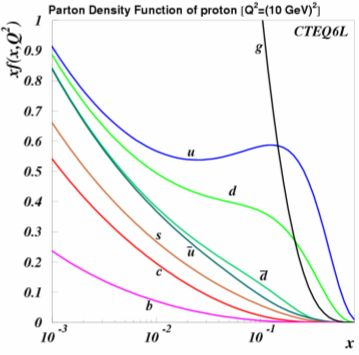
\includegraphics[width=0.5\textwidth]{1_Introduction_Th_and_Exp/pics/pdf.jpg}
\caption{Parton distribution function of the proton as a function of the Bjorken variable x, for a $Q^2=10$ GeV$^2$. }
\label{fig:pdf}
\end{figure}

As shown in figure \ref{fig:pdf}, the majority of the partons present in the protons are gluons, especially at low $x$. This effects directly translate in a dominance of the gluon-fusion process in the Higgs boson production at the LHC. The Feynman diagram showing the gluon fusion process can be found in figure \ref{fig:ggf}. The loop inside the gluon fusion process is dominated by the top quark, since it has the largest mass in the standard model, but may receive additional contribution from new physics. 

The second largest contribution to the total Higgs production cross section comes from the vector boson fusion (VBF) process (figure \ref{fig:vbf}) in which two quarks radiate two weak bosons that then interact producing a Higgs boson. The scattered quarks produce two jets in the forward/backward direction that can be used to experimentally tag the events.

The third most significant production mode is the associated production with a vector boson (VH, figure \ref{fig:vh}), also known as \emph{Higgsstralhung} process. The work presented in this thesis is focused on this production mechanism. Even though the production cross section is significantly lower than the previous two processes, the presence of a vector boson reduces greatly the background contamination. %This process is also the leading source of Higgs bosons at lepton colliders.

%Finally, the Higgs production in association with top quarks, $t\bar{t}$H (Figure \ref{fig:tth}), has the smallest cross-section with respect to the previous processes.
The most rare Higgs production process is $t\bar{t}$H, the production in association with top quarks (figure \ref{fig:tth}).

The cross sections of the four production processes depends on the mass of the Higgs boson, a free parameter of the SM, and on the center-of-mass energy of the two colliding beams. Figure \ref{fig:hxs} shows the production cross sections as a function of the Higgs mass at 7 and 8 TeV.

\begin{figure}
        \centering
        \begin{subfigure}[b]{0.3\textwidth}
                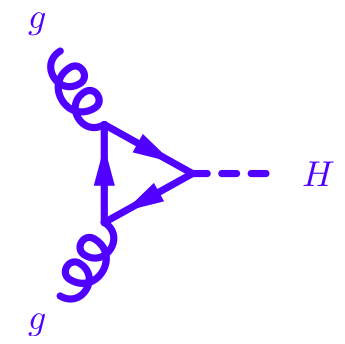
\includegraphics[width=\textwidth]{1_Introduction_Th_and_Exp/pics/ggFusion.png}
                \caption{Gluon fusion}
                \label{fig:ggf}
        \end{subfigure}%
        ~ 
        \begin{subfigure}[b]{0.3\textwidth}
                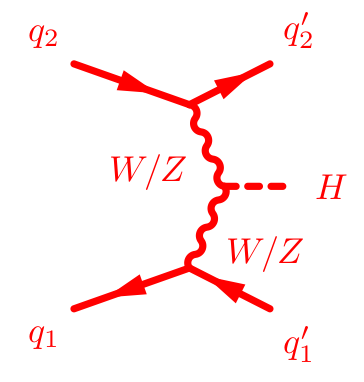
\includegraphics[width=\textwidth]{1_Introduction_Th_and_Exp/pics/BosonFusion.png}
                \caption{Vector boson fusion}
                \label{fig:vbf}
        \end{subfigure}

        \begin{subfigure}[b]{0.3\textwidth}
                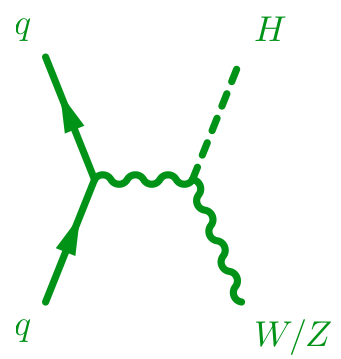
\includegraphics[width=\textwidth]{1_Introduction_Th_and_Exp/pics/Higgsstralhung.png}
                \caption{Associated production (Higgsstralhung) with vector boson}
                \label{fig:vh}
        \end{subfigure}
        ~ 
        \begin{subfigure}[b]{0.3\textwidth}
                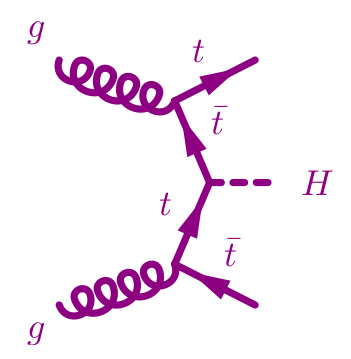
\includegraphics[width=\textwidth]{1_Introduction_Th_and_Exp/pics/ttFusion.png}
                \caption{$t\bar{t}$H}
                \label{fig:tth}
        \end{subfigure}
        \caption{Tree-level Feynman diagrams for the four Higgs boson production mechanisms relevant at LHC.}\label{fig:hprod}
\end{figure}

\begin{figure}
        \centering
	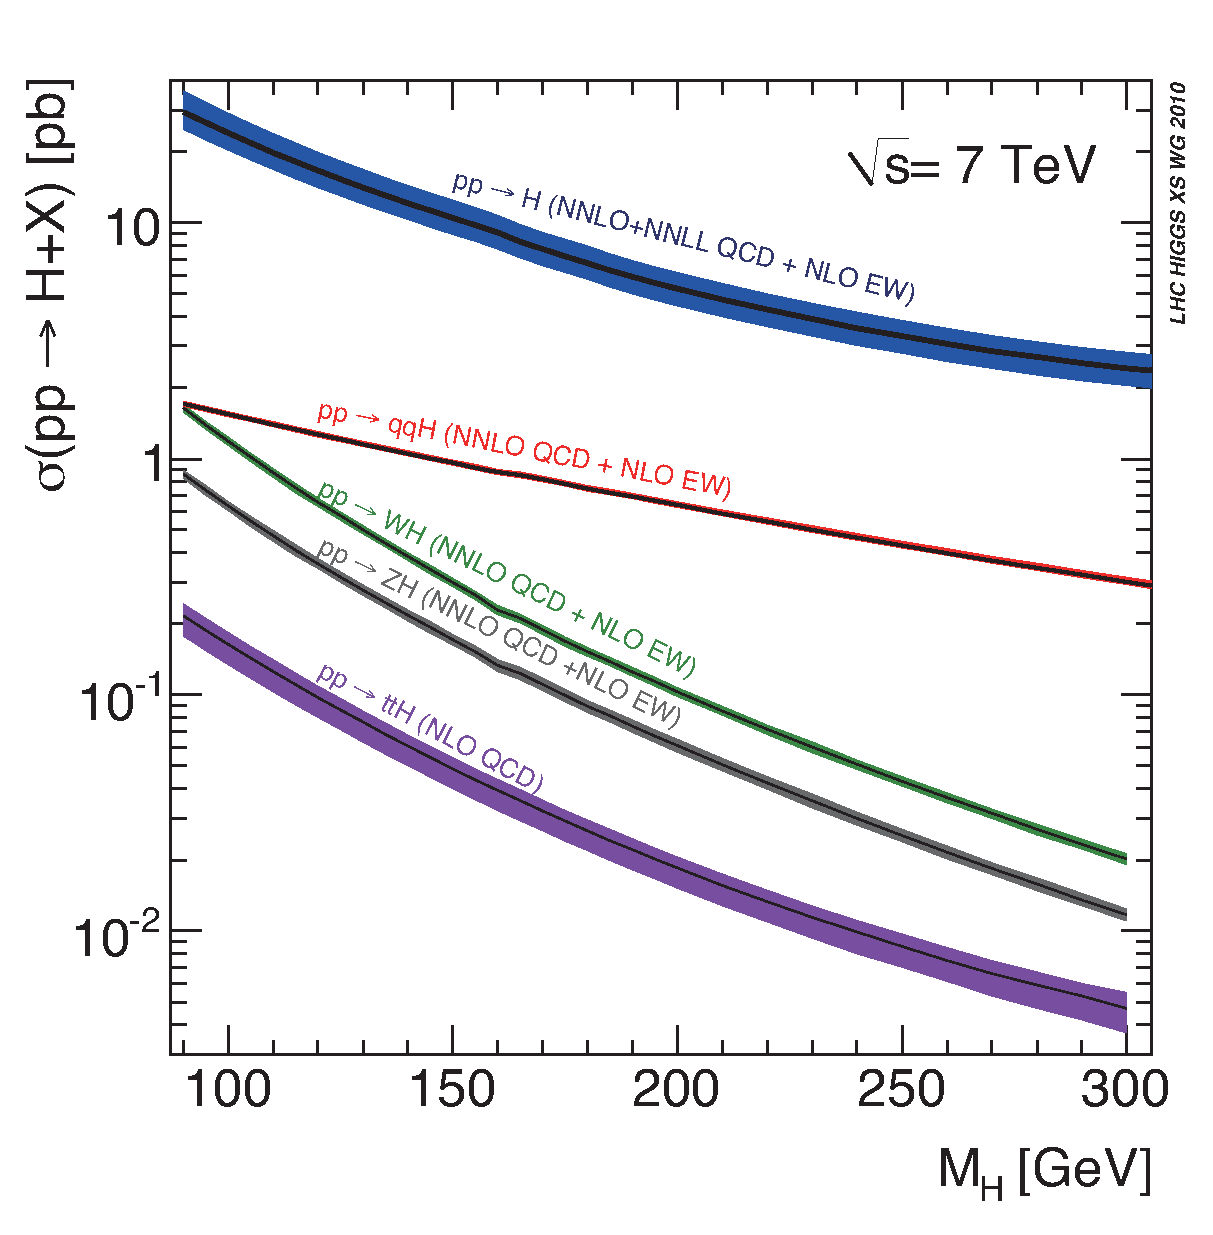
\includegraphics[width=0.48\textwidth]{1_Introduction_Th_and_Exp/pics/Higgs_XS_7TeV_LM.eps}
	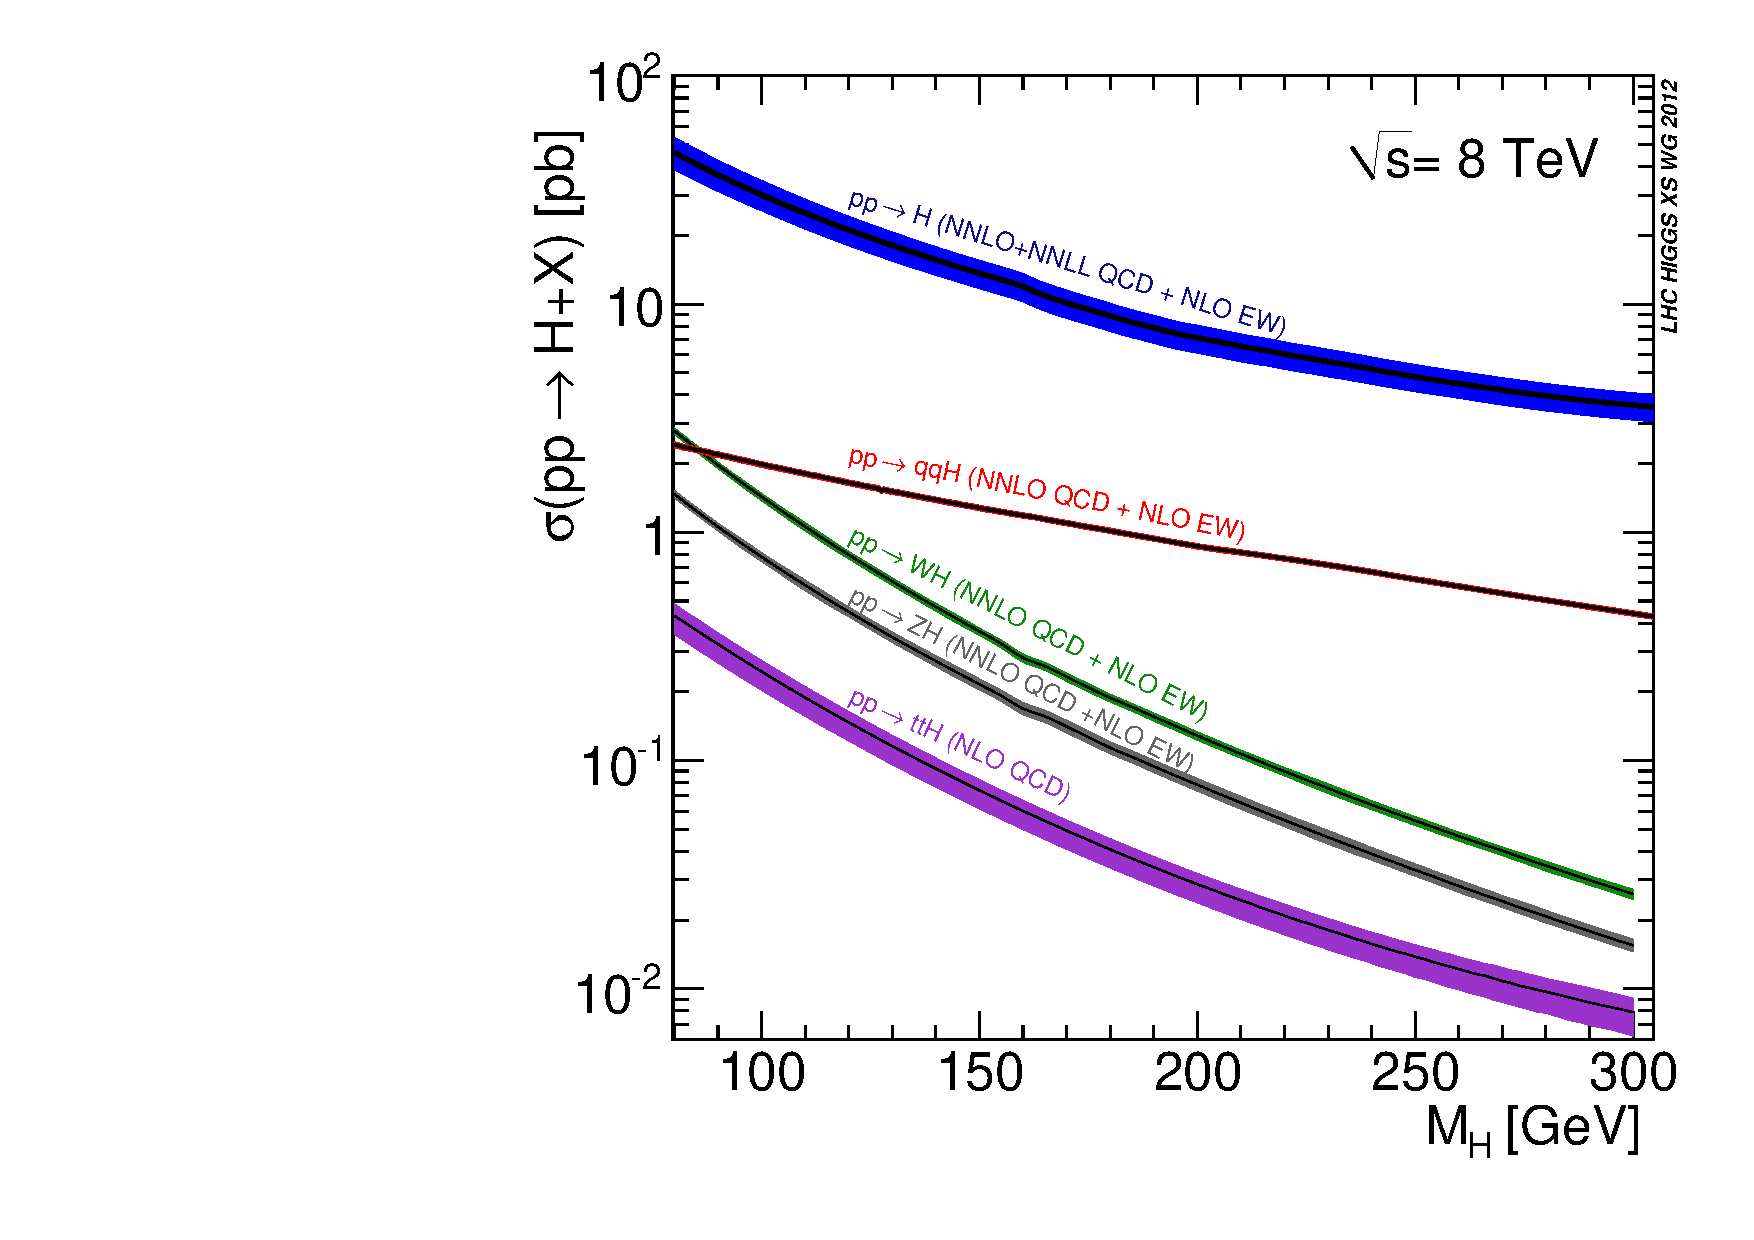
\includegraphics[width=0.48\textwidth]{1_Introduction_Th_and_Exp/pics/Higgs_XS_8TeV_LM.pdf}
       \caption{Higgs production cross section at 7 TeV (left) and 8 TeV (right). The bands represent the theoretical uncertainties~\cite{Heinemeyer:2013tqa}.}
       \label{fig:hxs}
\end{figure}


Even though the couplings of the Higgs boson are dictated only by the mass of the fundamental particles, the branching ratio of the Higgs boson to fundamental particles is also dependent on the Higgs mass, as a phase-space factor is added. The dependence of the branching fractions for the main Higgs decay modes as a function of its mass are shown in figure \ref{fig:hbr}. 

\begin{figure}
\centering
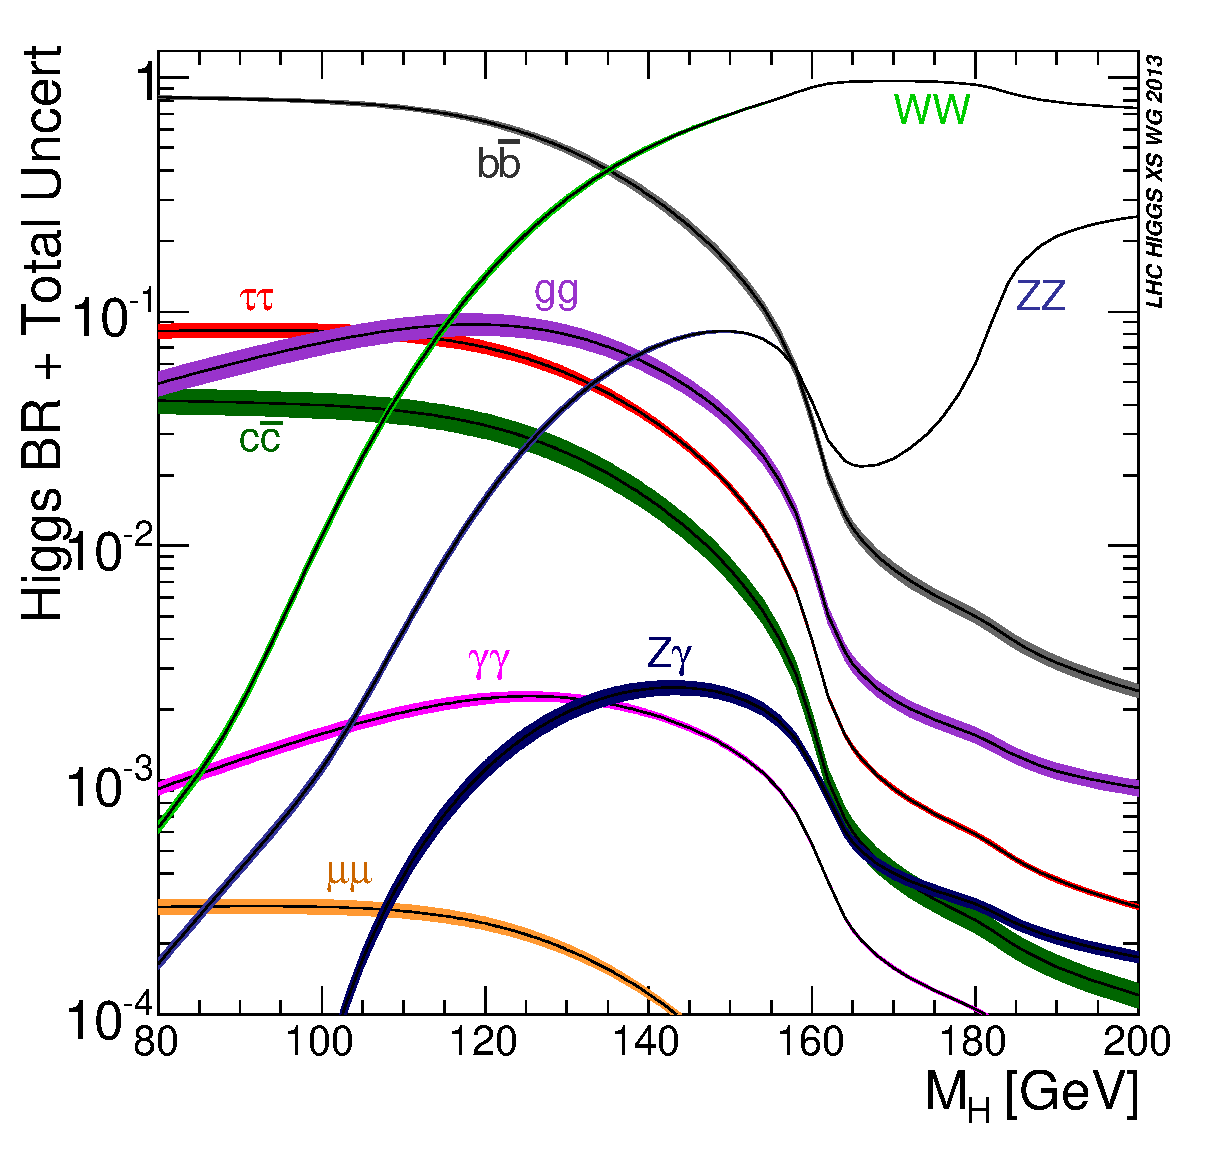
\includegraphics[width=0.5\textwidth]{1_Introduction_Th_and_Exp/pics/Higgs_BR_LM.eps}
\caption{Higgs branching ratios for different decay channels as function of the Higgs mass \cite{Heinemeyer:2013tqa}.}
\label{fig:hbr}
\end{figure}

Even though the Higgs boson has no direct coupling to the photon, a seizable branching ratio is given by loop contributions. These loops, as in case of the gluon fusion, could contain contributions from new physics, making this process a viable channel to probe theories beyond the standard model. The branching fraction to down-type fermions, may be sensitive to several beyond the Standard Model (BSM) models, in which these branching fractions are either enhanced or suppressed.

\section{Higgs boson searches}
\label{sec:higgs_res}

On the July 4$^{th}$ 2012, the CMS and ATLAS collaborations reported the observation of a new resonance at the mass of 125 GeV compatible with the SM Higgs boson \cite{Chatrchyan:2013lba}. This observation was based on combining the results of different searches for the Higgs boson in decay channels with gauge bosons, ZZ$^\ast$, WW$^\ast$ and $\gamma\gamma$.

Currently, the significance of the Higgs boson signal exceeds 5$\sigma$ for $\H\To\gamma\gamma$ searches in both CMS and ATLAS \cite{Khachatryan:2014ira, ATLASCONF:2014009}. A similar situation is also present in the ZZ$^\ast$ and WW$^\ast$ channels.

The large amount of signal events in these decay channels has allowed to perform initial studies of the resonance properties. The high invariant mass resolution of $\gamma\gamma$ and ZZ channels has allowed to measure the mass of the boson with high precision: $m_\H = 125.36 \pm 0.37\, \rm{(stat)} \pm 0.18\, \rm{(syst)}$ GeV and $m_\H = 125.03^{+0.26}_{-0.27} \,\rm{(stat)}^{+0.13}_{-0.15}  \,\rm{(syst)} = 125.03^{+0.29}_{-0.31} \, \rm{(tot)}$ GeV for ATLAS \cite{Aad:2014aba} and CMS \cite{CMS:2014ega}, respectively.

The spin and parity ($J^P$) of the resonance has also been studied in the ZZ and WW channels, which are more sensitive to these physical observables. The results, shown in Figure \ref{fig:hjp}, exclude any concurrent hypothesis at more than 99\% confidence level (CL), leaving only $0\+$ as an option \cite{CMS:2014gga}.

\begin{figure}
        \centering
	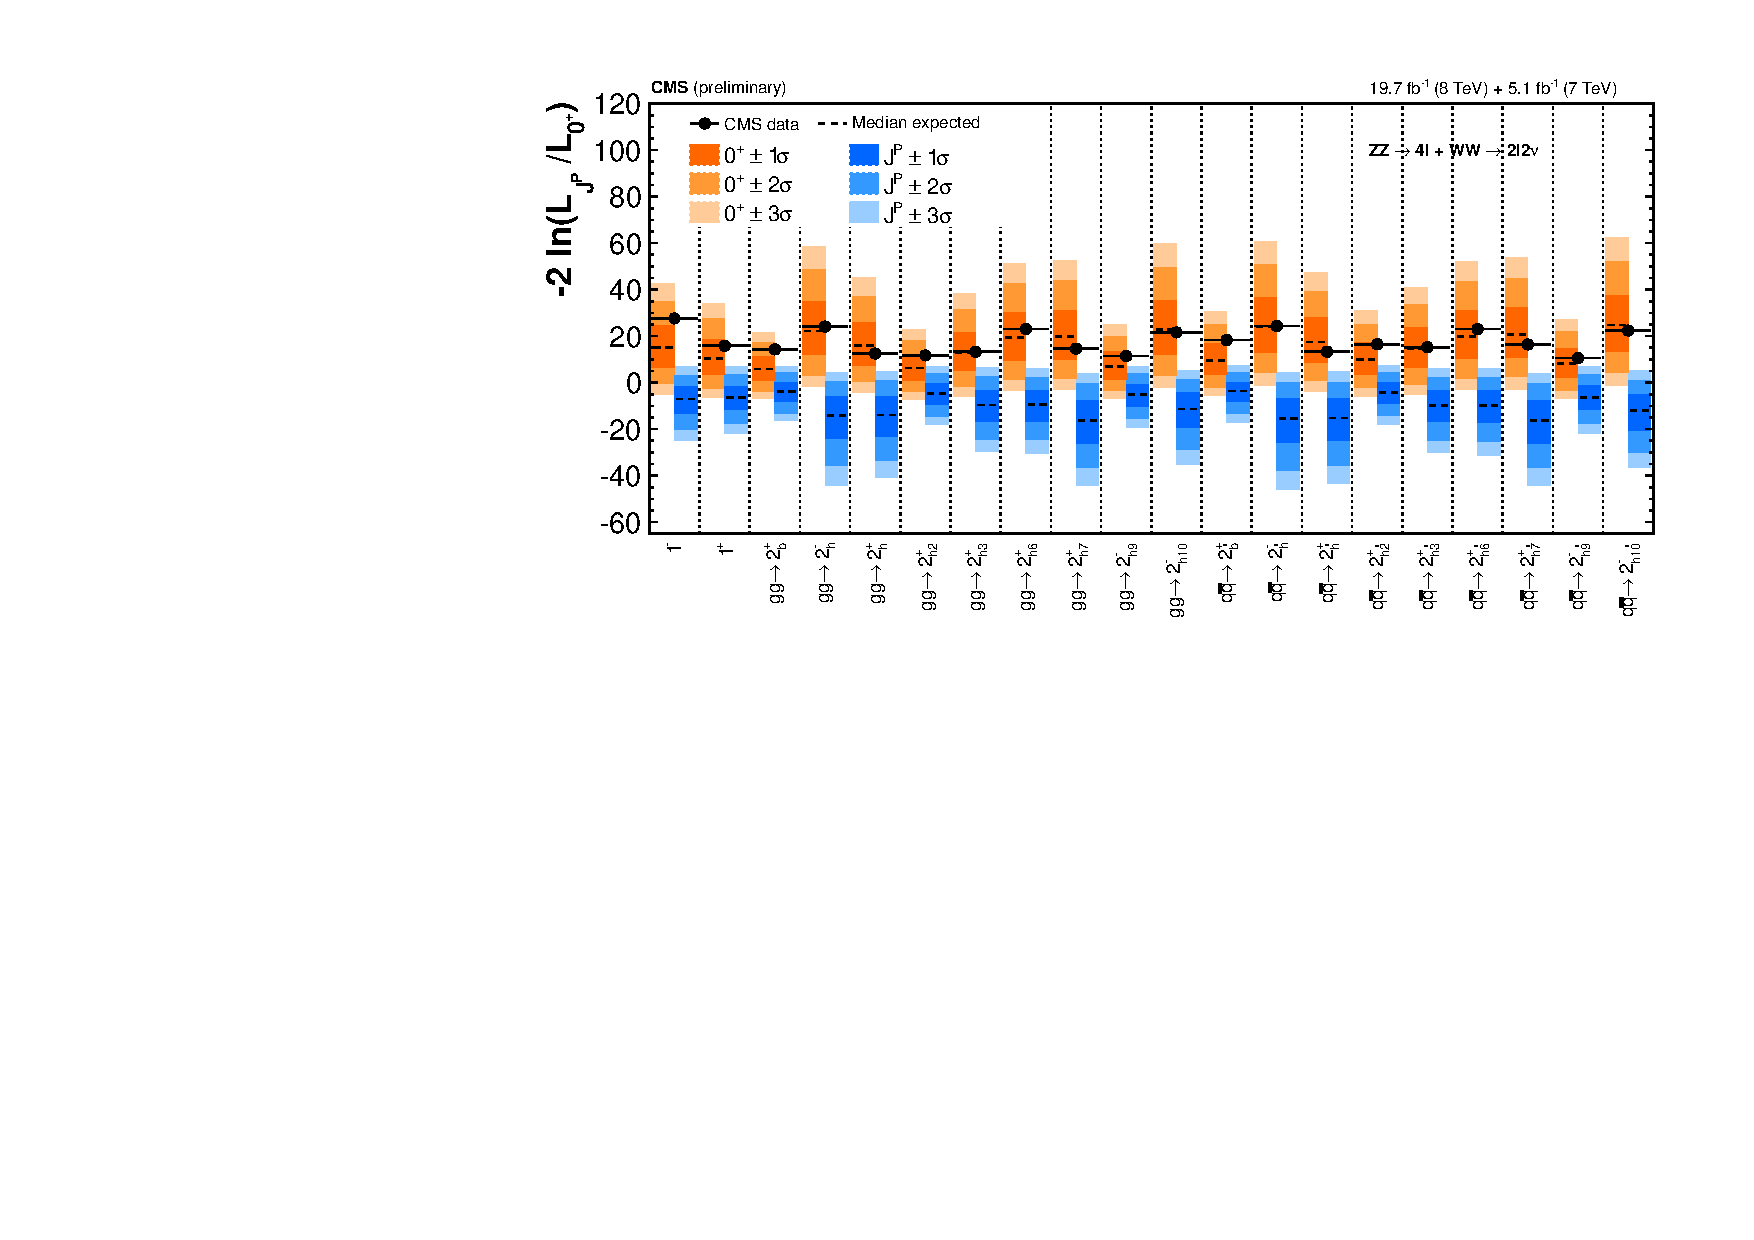
\includegraphics[width=0.8\textwidth]{1_Introduction_Th_and_Exp/pics/hwwhzz_JP_SummaryPlot.pdf}
       \caption{Summary of different $J^P$ hypotheses tested against the $0\+$ one using ZZ and WW Higgs candidate decays. The orange and blue bands represent the $1\sigma$, $2\sigma$, and $3\sigma$ around the median expected value for the SM Higgs boson hypothesis and the alternative hypothesis, respectively. The black points represent the observed values. }
       \label{fig:hjp}
\end{figure}

The expected SM Higgs boson width for $m_\H \approx 125$ GeV is $\Gamma_\H \approx 4$ MeV, which is below the experimental mass resolution. It has been pointed out that the ratio of on-shell and off-shell Higgs boson production cross section is proportional to the resonance width \cite{Caola:2013yja}; this effect is enhanced in the diboson decay channels by the interference term with the non resonant production. By simultaneously fitting the two contributions it has been possible to measure with better precision the 95\% CL upper limit on the width obtaining $\Gamma_{obs} / \Gamma_\H < 5.3$ for CMS \cite{Khachatryan:2014iha} and $\Gamma_{obs} / \Gamma_\H < 5.7$ for ATLAS \cite{ATLASCONF:2014042}. This method has mild model assumptions, as it neglects the contribution of new physics in the backgrounds and in the gluon-fusion loop. 

The search for Higgs boson decays to bottom quark pairs is the only feasible search to down-type quarks at hadronic colliders, as the coupling to the other two quarks are largely suppressed by their mass while the hadronic background increases dramatically. The large background contamination from heavy-flavor QCD production mandates to search for $\H\To b\bar{b}$ in the experimentally clean production processes such as the associated production with a vector boson, the VBF production, or the $tt$H associated production.
 %restricts the searches to all production processes but the gluon fusion, allowing for the richer final state to be used to remove most of the backgrounds.

The combination of the CDF and D0 results \cite{Aaltonen:2012qt} show a $3.1\sigma$ evidence of the $\rm{H} \To b \bar{b}$ decay mode. The CMS experiment reported a $2.1\sigma$ excess in the VH, $\rm{H} \To b \bar{b}$ production \cite{Chatrchyan:2013zna}, compatible with the SM predictions. The equivalent analysis for ATLAS does not show any excess \cite{TheATLAScollaboration:2013lia}, but is also less sensitive.

The branching fraction of the Higgs boson to muon pairs is predicted to be very low, therefore any excess might be a strong indication of new physics. Both ATLAS \cite{Aad:2014xva} and CMS \cite{CMS:2013aga} have performed a search for  $\rm{H} \To \mu \bar{\mu}$ decays, exploiting the extremely good dimuon mass resolution, without finding any significant excess. The analyses set an independent upper limit on the branching ratio of approximately 7 times the SM expectation.

The SM Higgs coupling to top quarks can only be observed through the $t\bar{t}$H associated production, since the Higgs boson mass forbids the decay of the Higgs into top quark pairs. The search for $t\bar{t}$H \cite{ATLASCONF:2014043,CMS:2014ega} is performed in many Higgs final states. Both ATLAS and CMS exploit the $b\bar{b}$ and $\gamma\gamma$ final states; additionally CMS searches for this production mode also in multi-lepton final states, targeting the $\tau\tau$, ZZ, and WW Higgs decay modes.

The combination of these $tt$H searches leads in CMS to a $3.5\sigma$ excess with respect to the background-only hypothesis \cite{CMS:2014ega}. The combined \emph{signal strength} ($\mu$), i.e. the ratio $\mu = (\sigma \times BR)_{obs} / (\sigma \times BR)_{SM}$, is measured to be $\mu = 2.76^{+1.05}_{-0.92}$, which is two standard deviations away from the SM expectation ($\mu = 1$). The excess in this combination is driven by the same-sign dimuon analysis, which searches for $\H\To \W\W$. The results from ATLAS are consistent with the background-only hypothesis \cite{ATLASCONF:2014043}.

The $\H \to \tau \tau$ decay mode is searched by CMS in gluon fusion, VBF and associated production \cite{H_tautau}. Events are selected in real time by dedicated triggers and according to the isolation of the final state leptons. Events are separated into categories tailored around specific production mechanisms (VBF, VH, gluon fusion) and, in the gluon fusion case, according to the boost of the hadronic tau and Higgs candidates. The invariant mass spectrum of the Higgs final states is smeared due to the presence of neutrinos in the tau lepton decay. To recover this effect, a dedicated likelihood integration method, called SVFit~\cite{Bianchini:2014vza}, calculates the di-tau invariant mass taking as input the momenta of the visible Higgs products plus the information on the reconstructed missing transverse energy (\MET). The mass resolution achieved by SVFit varies between 10\% and 20\%, depending on the final state and the category.

Most of the backgrounds present in the direct production (VBF and gluon fusion) categories are modeled using simulated events with dedicated sideband regions to cross-check the simulation and apply correction factors where needed. The main background for these categories is given by $\Z \To \tau\tau$ events which are modeled with the embedding techniques~\cite{CMS_AN_2011-020}: real $\Z \To \mu \mu$ events are selected from collision data and the two muons are replaced with simulated tau decays.

The search for the Higgs boson in the associated production process is performed in final states including both a Z and a W boson. These searches exploit the presence of the additional leptons in the final state to suppress the backgrounds. The remaining backgrounds are estimated with MC simulation or with the misidentification rate method. Part of the work presented in this thesis has been included in the final result published by the collaboration, but additional effort has been put into estimating the uncertainties in one of the major sources of backgrounds. 

A combined fit to all the channels and categories of the CMS $\rm{H} \To \tau\tau$ analysis reveals a $3.2\,\sigma$ deviation from the background-only hypothesis and a combined $\mu = 0.78 \pm 0.27$. %, well compatible between channels, as shown in Figure \ref{fig:htt_mu}. 
The best-fit mass, $m_\H = 122 \pm 7$ GeV, is compatible with the Higgs mass measured in the ZZ and $\gamma\gamma$ decay channels. The equivalent ATLAS analysis \cite{ATLASCONF:2013108}, which lacks the associated production search, observes a $4.1\,\sigma$ deviation from the background-only hypothesis and measures $\mu = 1.4^{+0.5}_{-0.4}$, which is slightly in excess, but still compatible, with respect to the SM value.

The CMS $\H \To b\bar{b}$ and $\H \To \tau \tau$ searches have been combined leading to a $3.8\,\sigma$ evidence of Higgs coupling to down-type fermions \cite{Chatrchyan:2014vua}.

The result of the single and combined signal strengths for both ATLAS \cite{ATLASCONF:2014009} and CMS \cite{CMS:2014ega} is presented in Figure \ref{fig:combination}.
The outcome of the various searches have been combined by the single experiments in a simultaneous fit in order to determine the couplings of the Higgs boson to the different types of particles. 

\begin{figure}
        \centering
	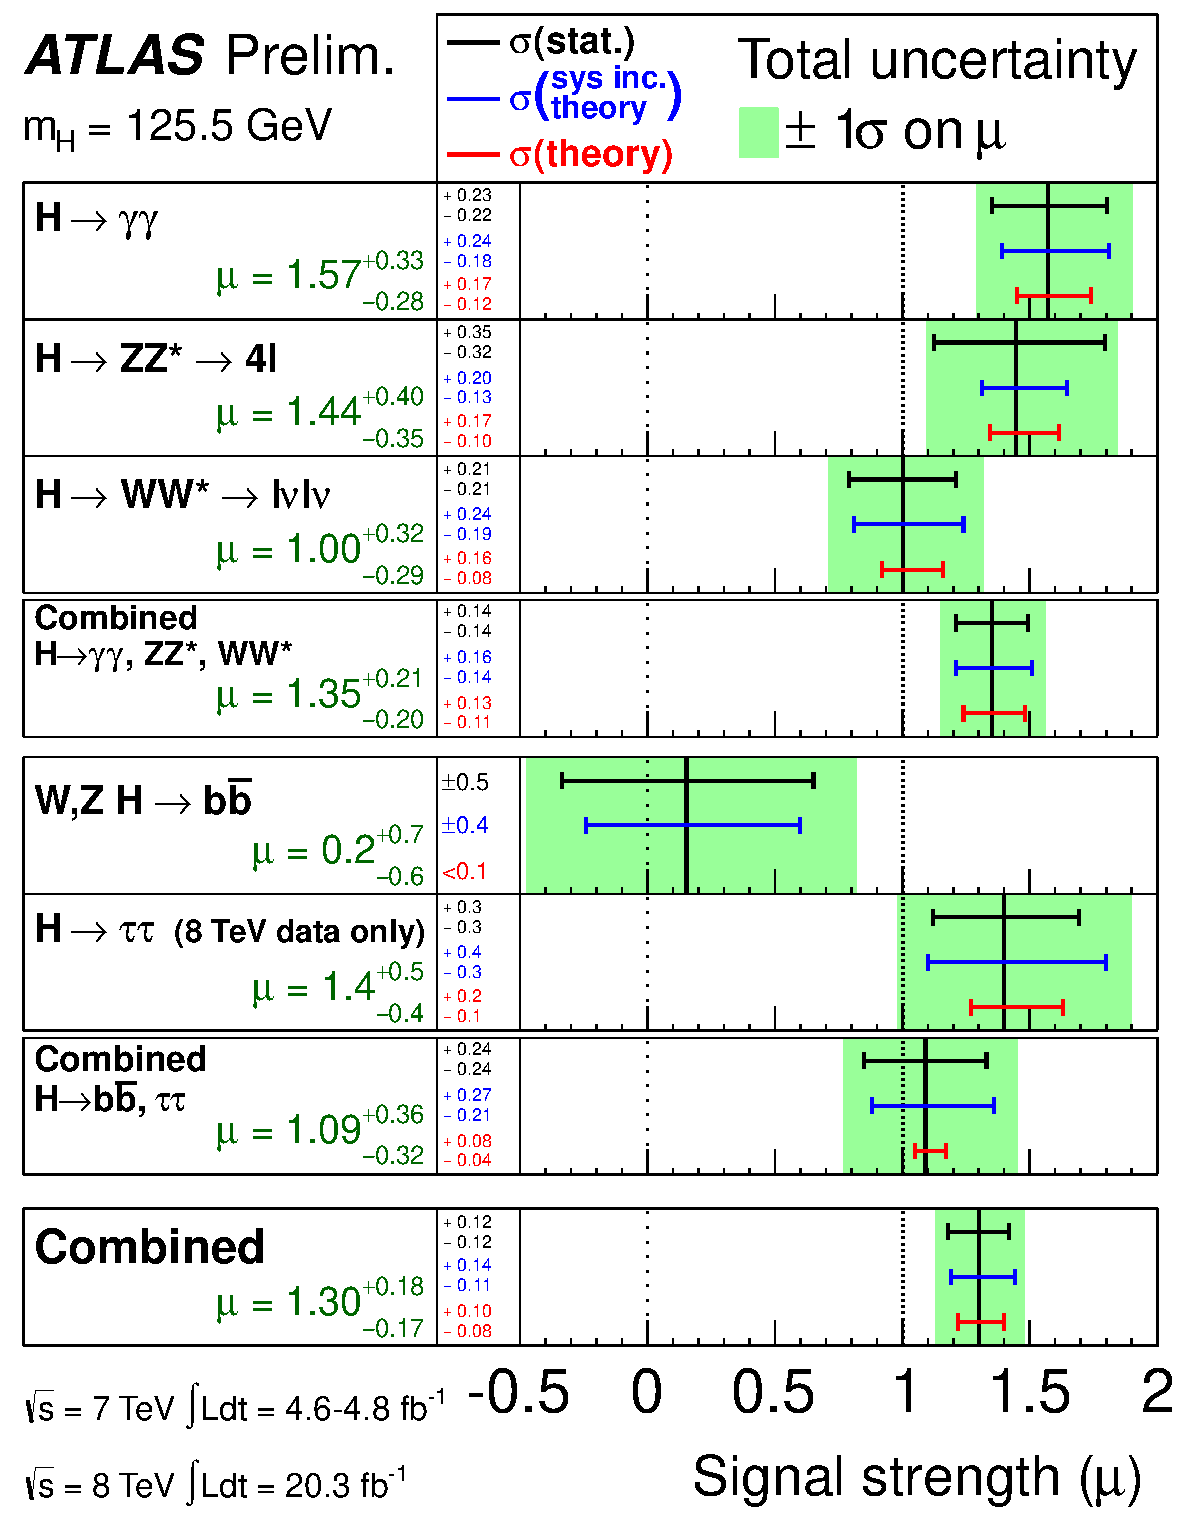
\includegraphics[width=0.39\textwidth]{1_Introduction_Th_and_Exp/pics/fig_01.pdf}
	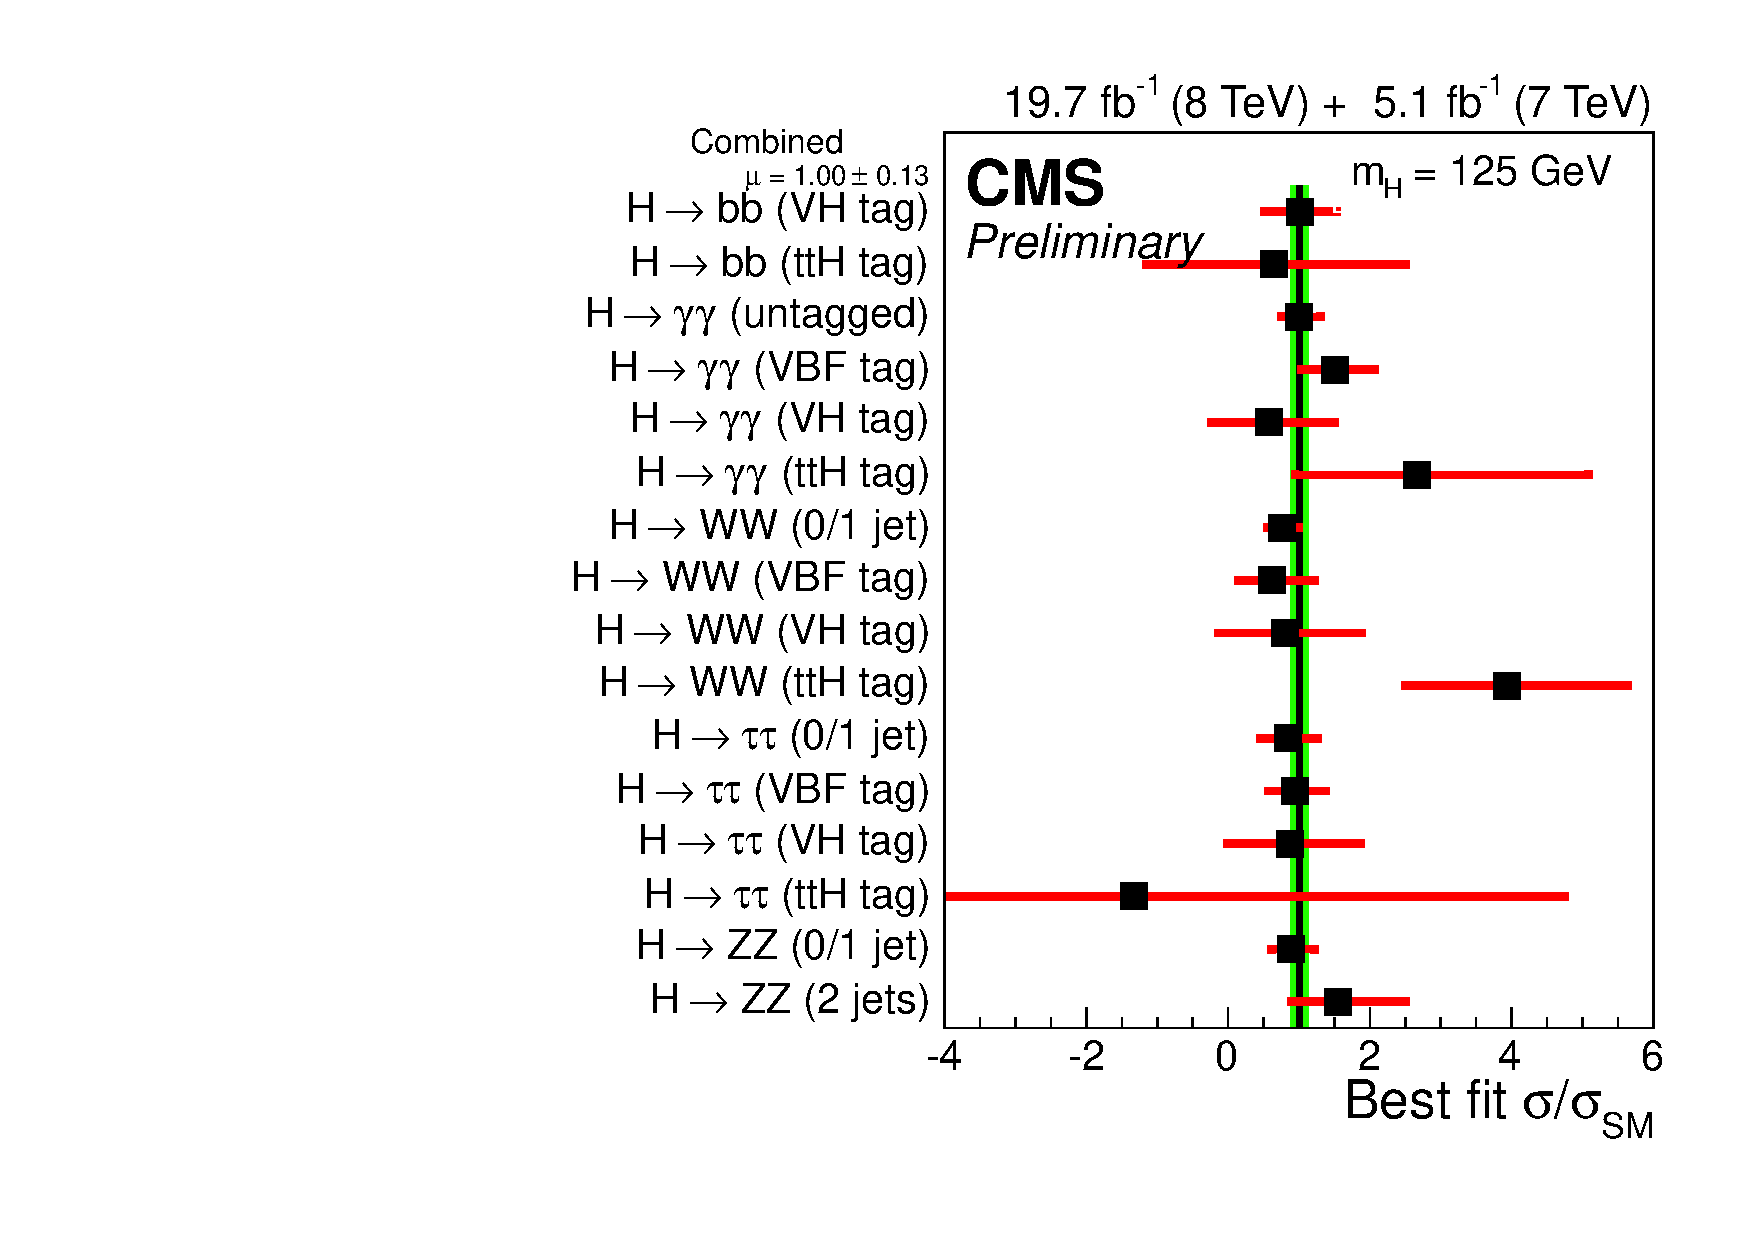
\includegraphics[width=0.54\textwidth]{1_Introduction_Th_and_Exp/pics/sqr_mlz_ccc_mH125.pdf}
       \caption{Overview of the different Higgs boson searches performed by ATLAS (left) and CMS (right) with the respective signal strength measured by each channel. The combined result is $\mu = 1.30^{+0.18}_{-0.17}$ for ATLAS and $\mu = 1.00 \pm 0.13$ for CMS.}
       \label{fig:combination}
\end{figure}

Another way to interpret the results is to compute the couplings of the Higgs boson to gauge bosons ($k_V$) and to fermions ($k_F$) and to plot the one-sigma contour regions allowed by each measurement. This interpretation assumes the absence of new physics in loop processes to infer the two couplings from the measurements (e.g. assumes that the gluon fusion is almost completely mediated by a top loop). This interpretation of the results is available in Figure \ref{fig:kvf} for both the experiments.

\begin{figure}
        \centering
	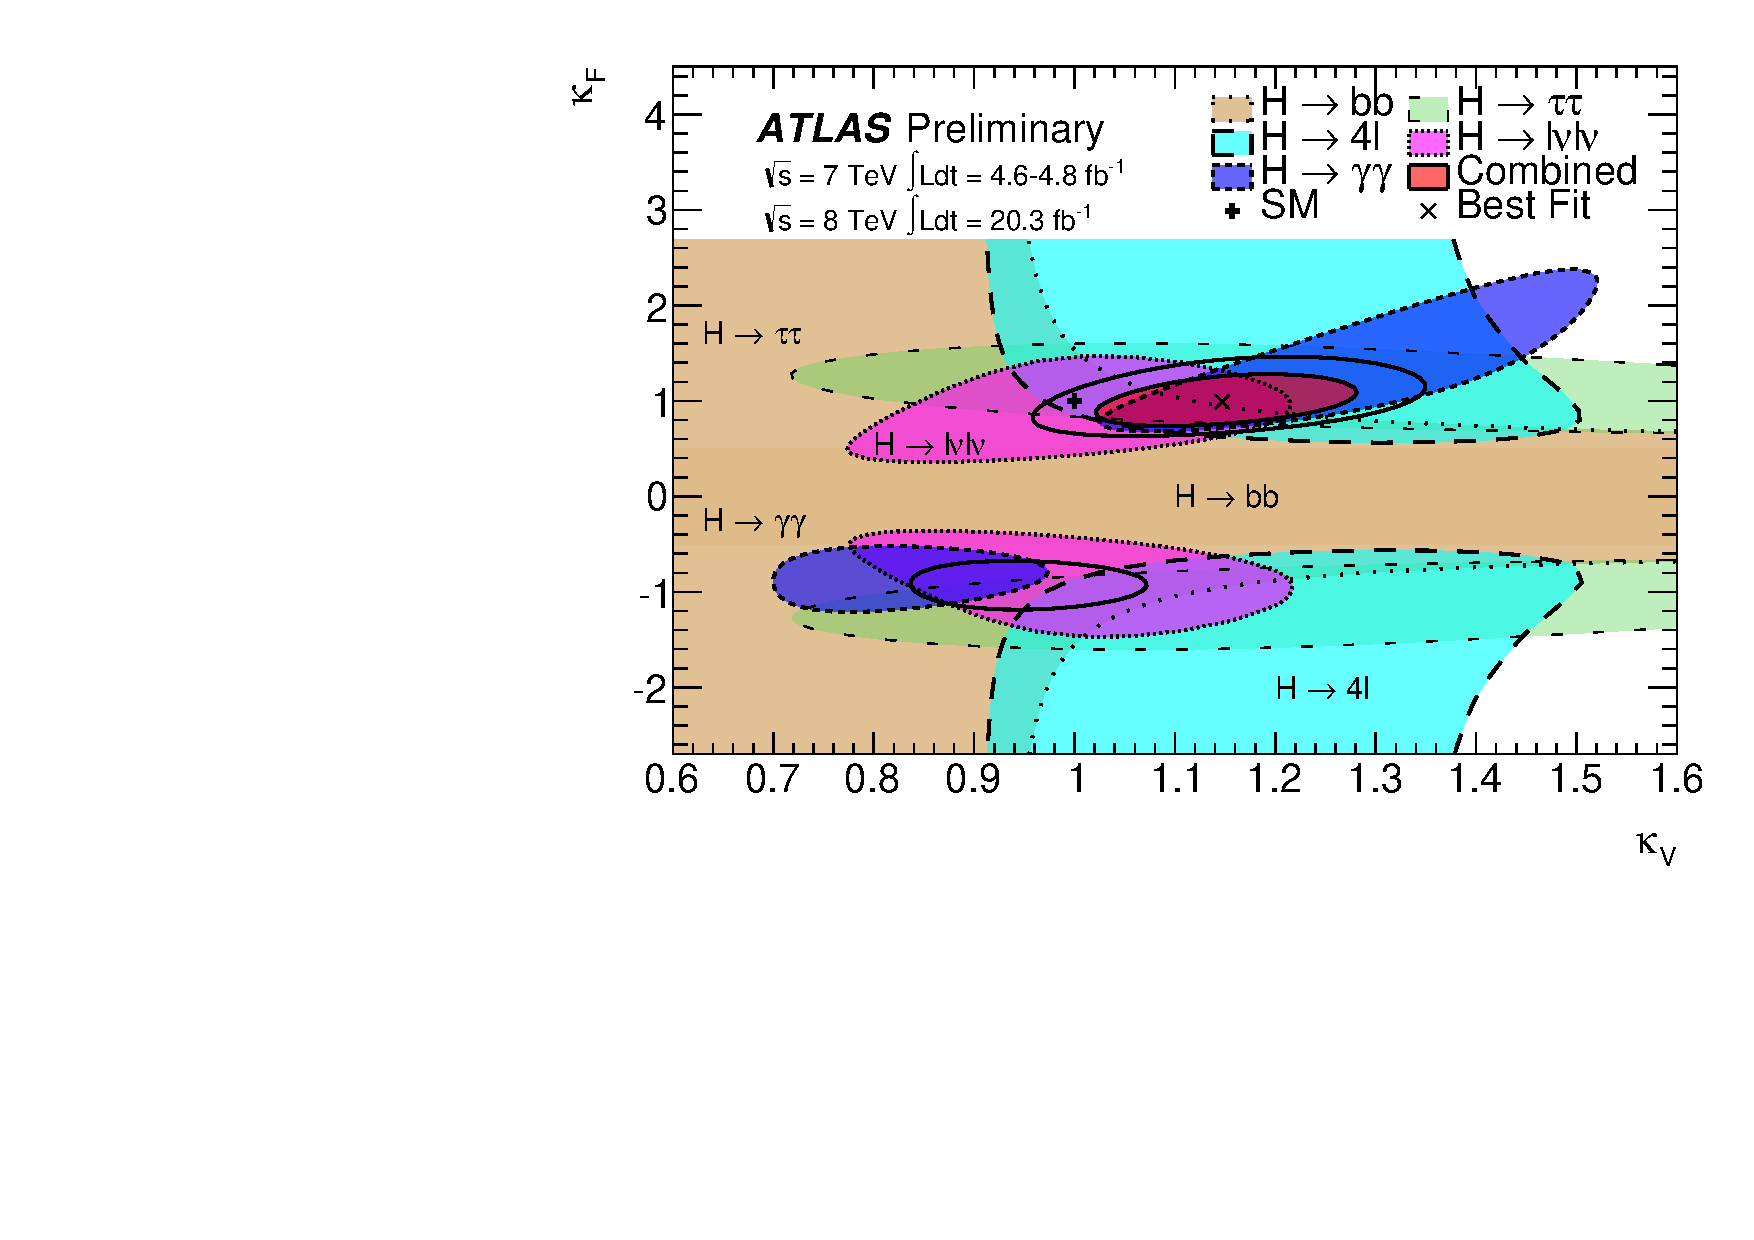
\includegraphics[width=0.53\textwidth]{1_Introduction_Th_and_Exp/pics/fig_05b.pdf}
	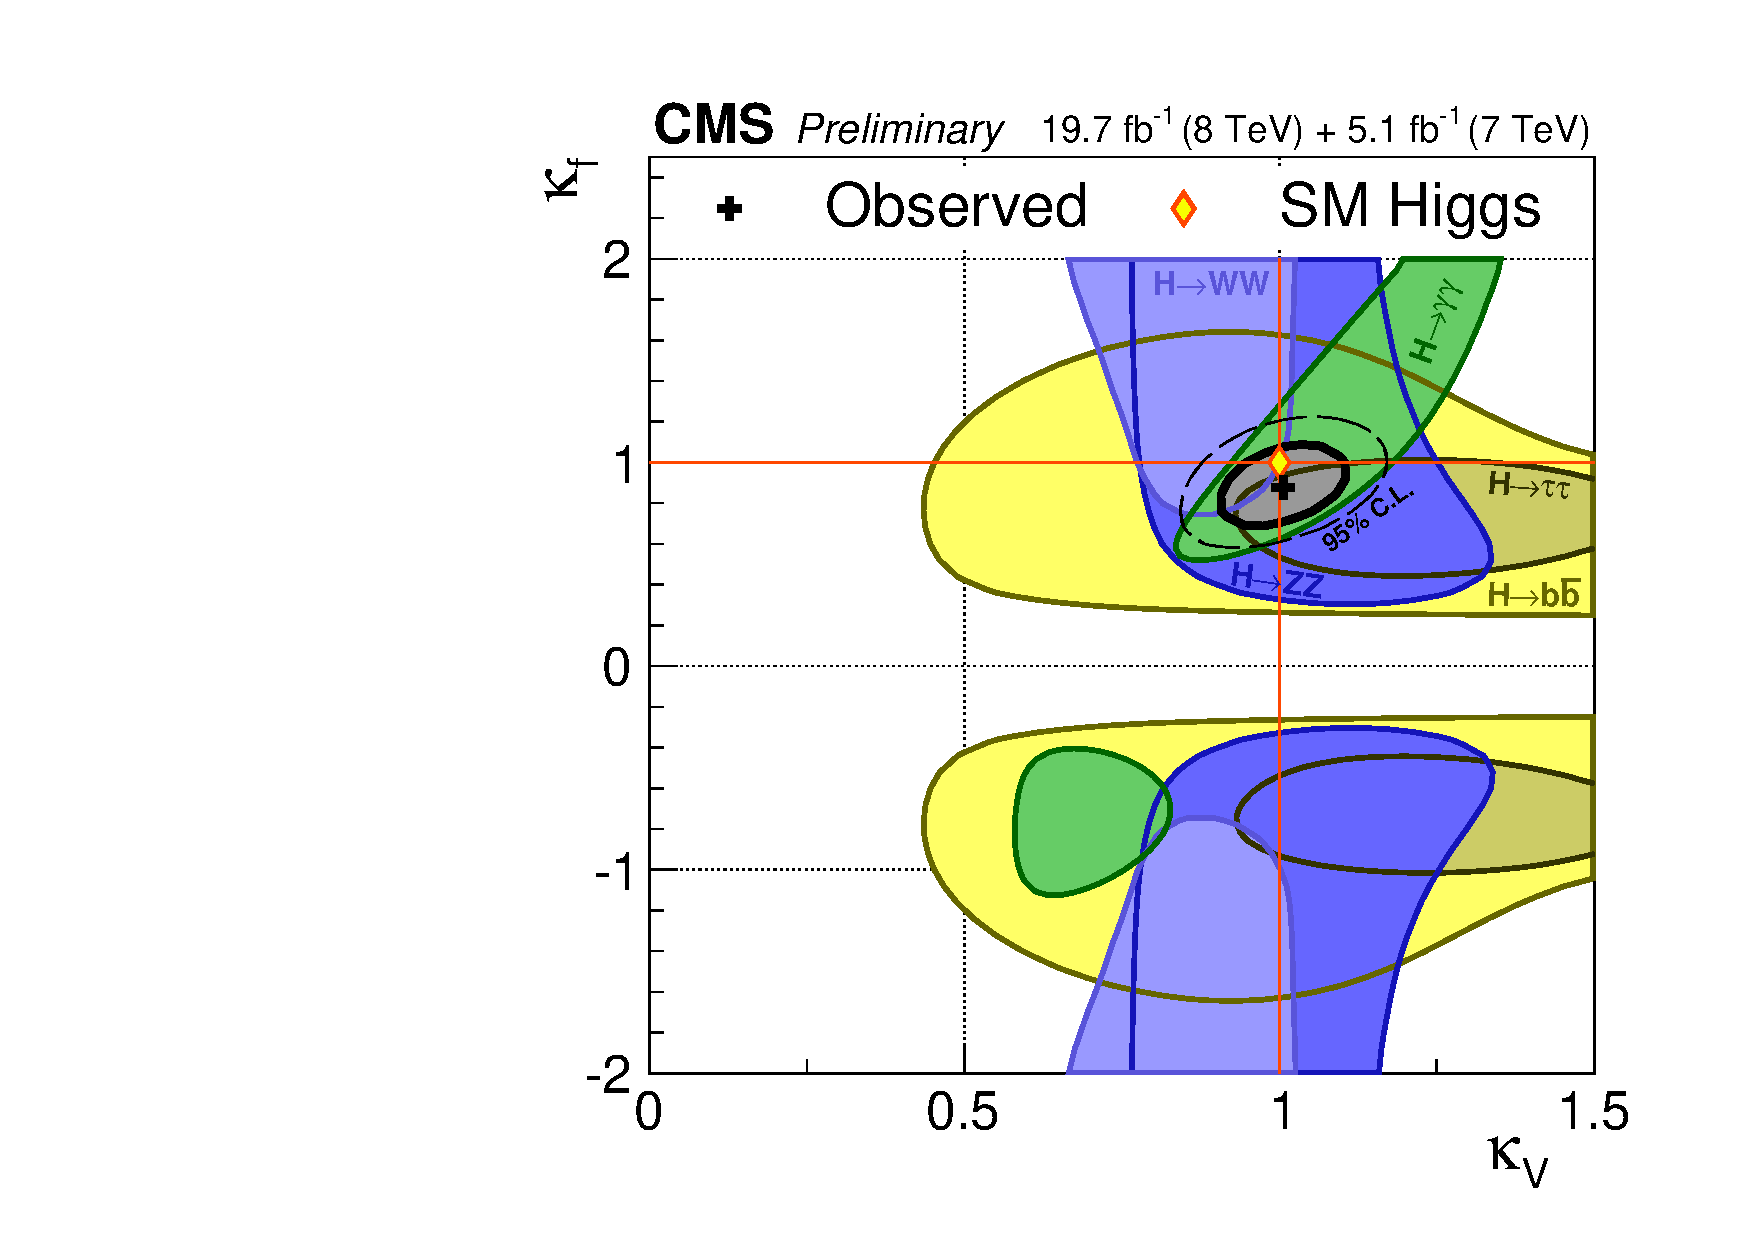
\includegraphics[width=0.41\textwidth]{1_Introduction_Th_and_Exp/pics/cVcF_all_channels_2quadrant.pdf}
       \caption{Allowed regions in the $k_V \times k_F$ space as measured by the different Higgs boson searches at ATLAS (left) and CMS (right). The colored contours represent the one standard deviation confidence intervals measured by the different searches and by their combinations. The best fit value of the couplings is marked by the symbol $\times$ (left) and by the black cross (right). The Standard Model point is located at (1, 1) and marked as a black cross on the left and as a yellow diamond on the right. }
       \label{fig:kvf}
\end{figure}

All the results reported so far by both ATLAS and CMS are compatible with the interpretation of the new resonance being a purely SM Higgs boson, but the accuracy of the measurements still allows room for new physics processes.

%In the following part of this work a more detailed description of the $\W\H \To \ell \ell \tau$ analysis will be shown. This 


